% Conteúdo comum aos três estilos (capa + slide de exemplo)
\setbeamerfont{itemize/enumerate body}{size=\small}
\newcommand{\titulotg}{Análise da influência de parâmetros de processo de fabricação (cinemáticos, de geometria da ferramenta, entre outros) na integridade de juntas soldadas por FSW}
\newcommand{\subtitulotg}{Coeficiente Analítico de Vazio ($C_{void}$) para a previsão de vazios volumétricos}
\newcommand{\autortg}{Rafael Lucas de Albuquerque Louvain}
\newcommand{\orientadortg}{Orientador: Prof. Dr. Lindolfo Araújo Moreira Filho}
\newcommand{\infotg}{Trabalho de Graduação 2 \;$\cdot$\; Engenharia Mecânica-Aeronáutica \;$\cdot$\; ITA \;$\cdot$\; 2026}

\newcommand{\slideexemplo}{%
\begin{frame}{Abordagem 2: velocidade periférica crítica do ombro}
\begin{columns}[T,onlytextwidth]
\begin{column}{0.47\textwidth}
\begin{itemize}\setlength{\itemsep}{5pt}
  \item \textbf{Índice:} $C_{void} = V_{crit}/(\omega R_s)$; prevê-se vazio quando $\omega R_s < V_{crit}$, isto é, quando falta calor junto ao ombro.
  \item \textbf{Limiar calibrado:} $V_{crit} = 0{,}84$~m/s, ou rotação (rpm) $\times$ raio do ombro (mm) $\approx 8.000$.
  \item \textbf{Desempenho:} 90,0\% no protocolo de Du et al. (27 de 30 soldas) e 72,9\% na média de 500 sorteios, acima da meta de 70\%.
  \item \textbf{Simplicidade:} um único parâmetro, sem simulação; o avanço e a pressão não entram na expressão.
\end{itemize}
\end{column}
\begin{column}{0.5\textwidth}
\centering
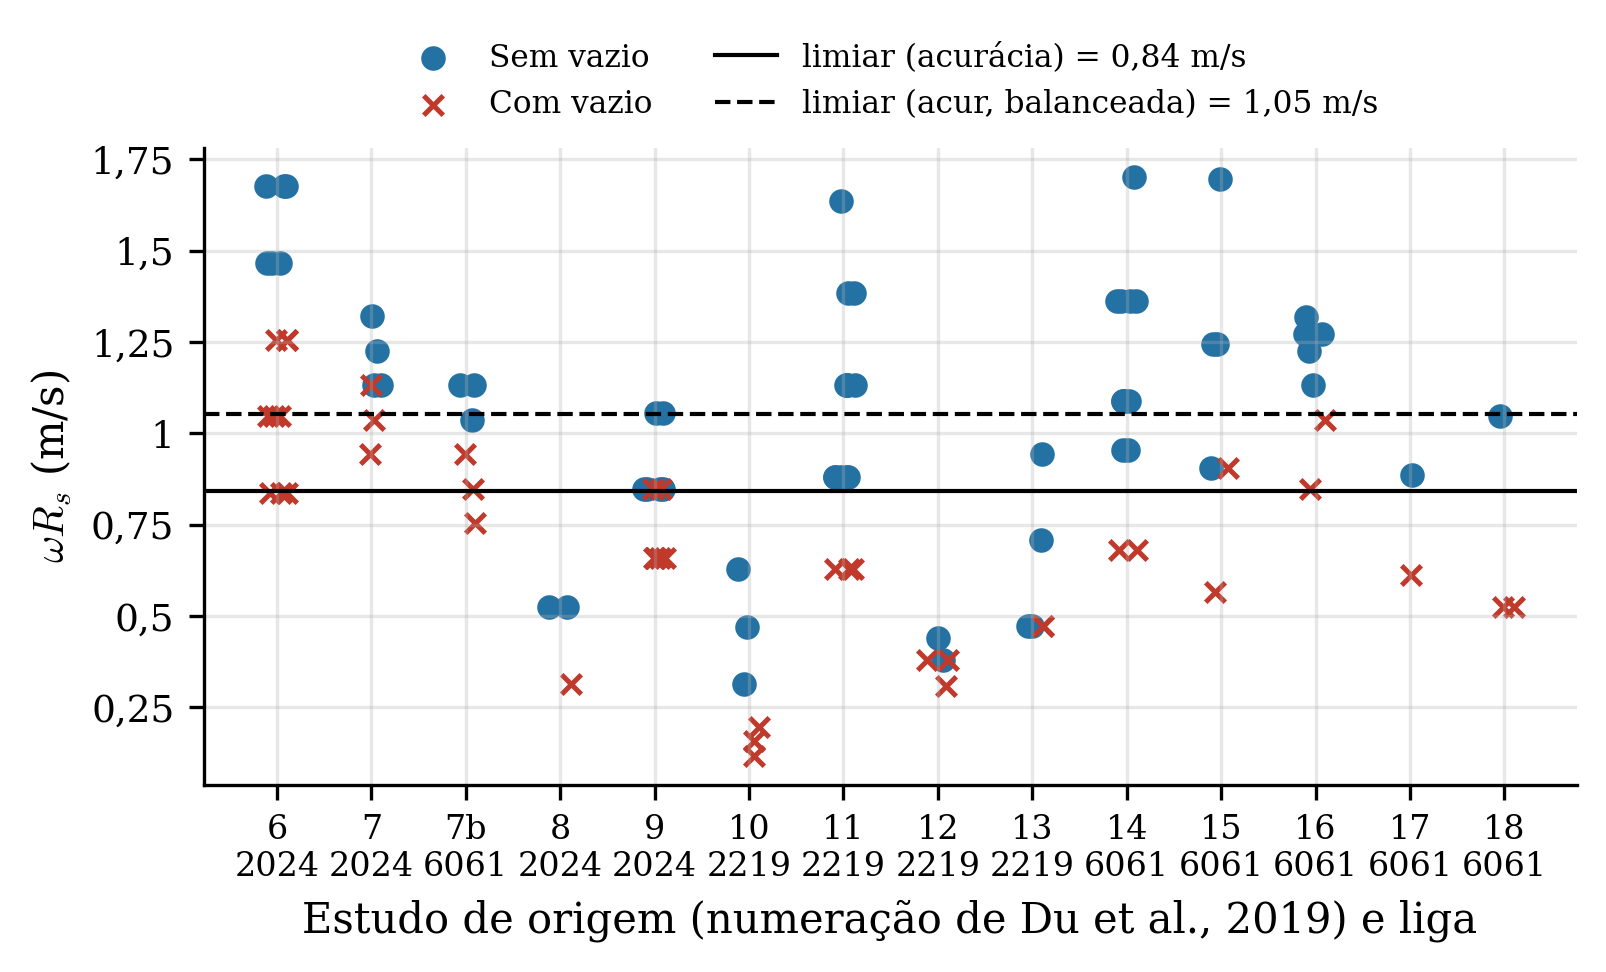
\includegraphics[width=\linewidth]{fig-r-indice-wrs.png}\\[2pt]
{\scriptsize Soldas abaixo da linha cheia: vazio previsto.}
\end{column}
\end{columns}
\end{frame}}
